\documentclass[aspectratio=43]{beamer}
%Information to be included in the title page:
\title{Paper Reading}
\author{Dachun Kai}
\institute{USTC}
\date{August 6, 2021}
%\usetheme{CambridgeUS}
\usetheme{Boadilla}

\usepackage[backend=bibtex,sorting=none]{biblatex}
%\usepackage{ctex}
\addbibresource{ref.bib} %BibTeX数据文件及位置
\setbeamerfont{footnote}{size=\tiny}

\begin{document}
    \frame{\titlepage}
    
    \begin{frame}
    	\frametitle{Outline}
    	\tableofcontents
    \end{frame}
	
	\section{Paper 1: EFI-Net: Video Frame Interpolation from Fusion of Events and Frames}
	
	\begin{frame}
		\frametitle{Paper 1: EFI-Net\textit{(CVPR2021W)}}
		\begin{figure}
			\centering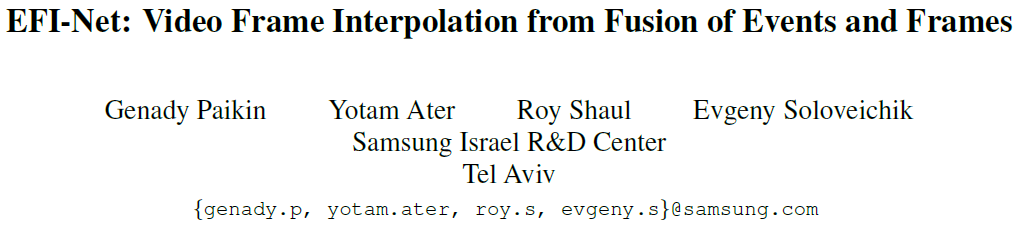
\includegraphics[width=0.95\linewidth]{images/EFI_NET_paper.png}
		\end{figure}
	\end{frame}

	\begin{frame}{Problem Definition}
		\only<1>{
			Classical CNN-based VFI(Video Frame Interpolation) methods, DAIN\footfullcite{bao2019depth} and SSM\footfullcite{jiang2018super} suffer from \alert{Occlusion}.
			\begin{figure}
				\centering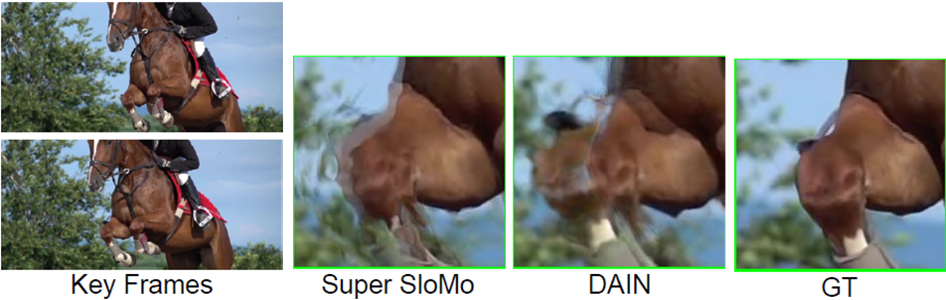
\includegraphics[width=0.9\linewidth]{images/occlusion.png}
			\end{figure}
		}
	
		\only<2>{
			DSM(Deep Slow Motion)\footfullcite{paliwal2020deep} fuse \alert{High-Resolution}, \alert{Low Frame Rate(Main Video)} with \alert{Low-Resolution} but \alert{High Frame Rate(Auxiliary Video)}.
			\begin{figure}
				\centering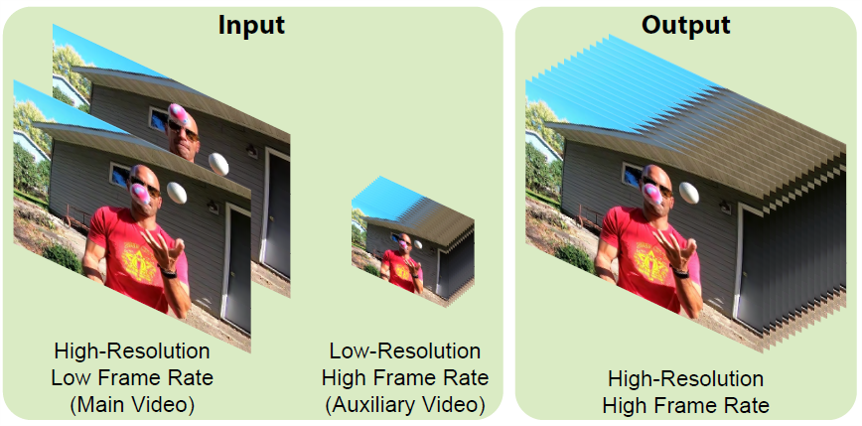
\includegraphics[width=0.8\linewidth]{images/DSM.png}
			\end{figure}
		}
	
		\only<3>{
			Great performance of Event Camera
			\begin{figure}
				\centering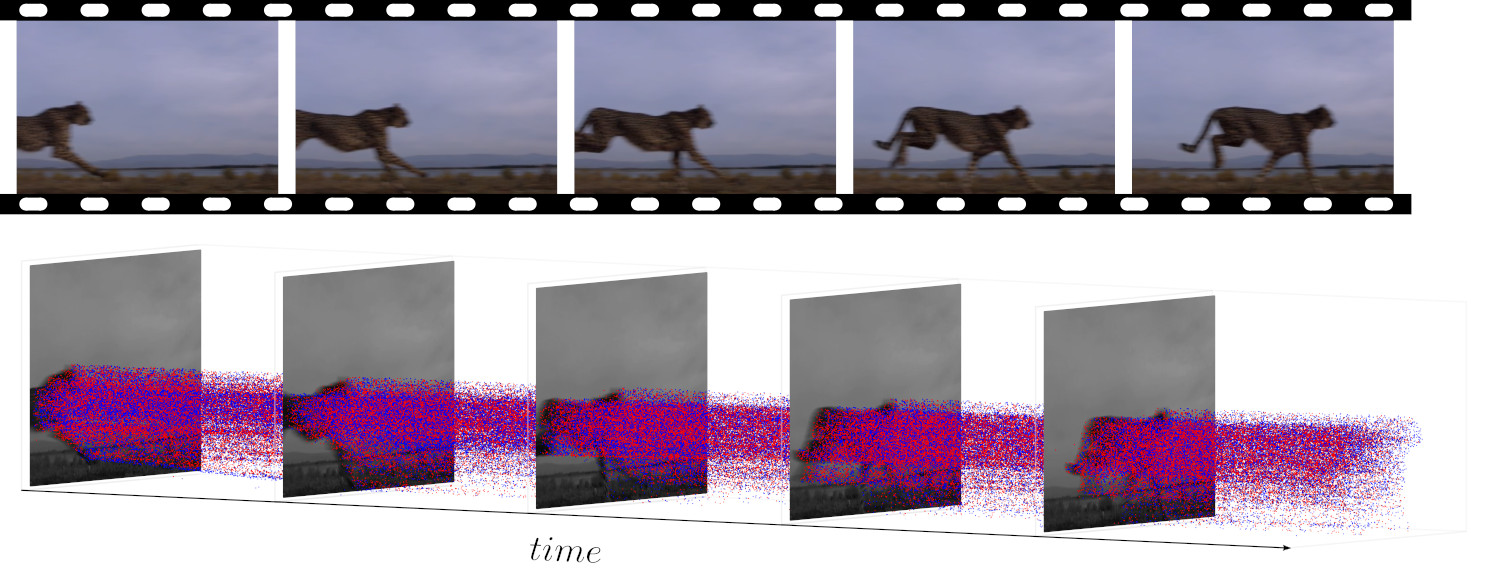
\includegraphics[width=0.85\linewidth]{images/Event_camera_comparison.jpg}
			\end{figure}
			\begin{itemize}
				\item High temporal resolution(microsecs)
				\item Low Latency
				\item Low Power(SNN, neuromorphic chip)
				\item No motion blur
				\item High dynamic range
			\end{itemize}
		}
	\end{frame}

	\begin{frame}{Proposed Method}
		\only<1-4>{The architecture of proposed EFI-Net
				\begin{figure}
					\centering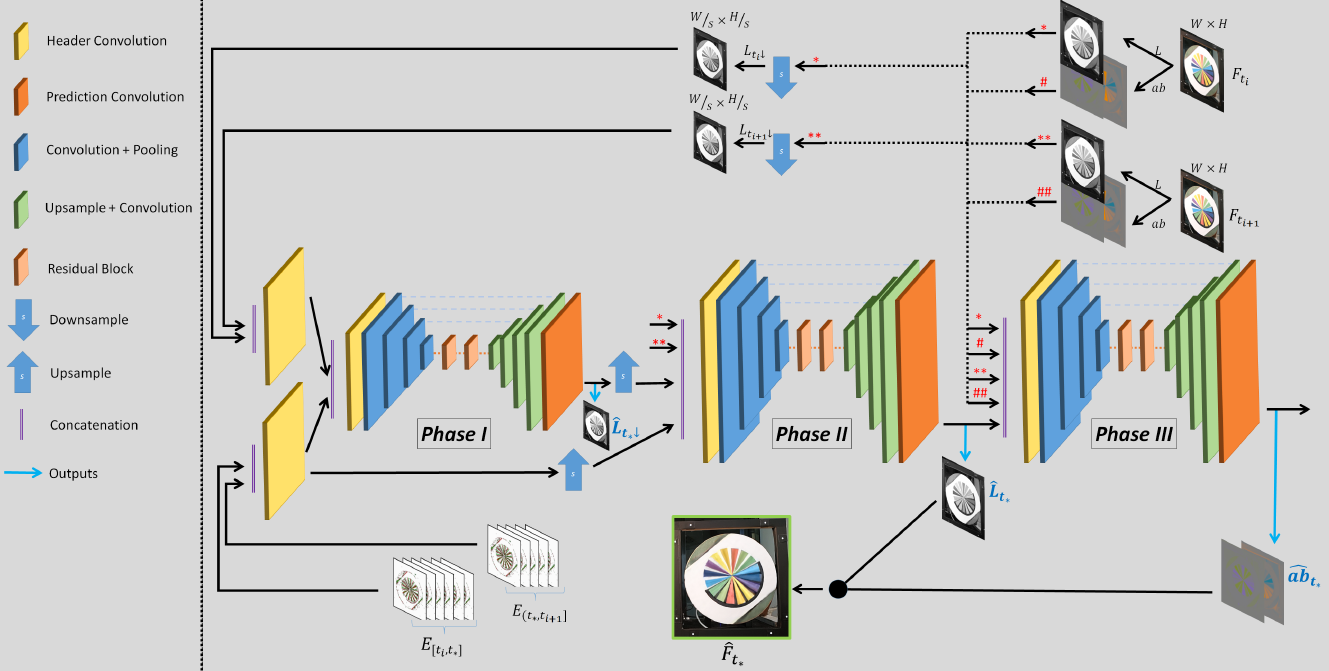
\includegraphics[width=0.9\linewidth]{images/EFI_NET_architecture.png}
				\end{figure}
		}
		\only<1>{
			\begin{itemize}
				\item Phase I: \alert{Low resolution} intensity interpolation
				\item Phase II: \alert{High resolution} intensity interpolation
				\item Phase III: \alert{Re-colorization}
			\end{itemize}
		}
		\only<2>{
			\begin{itemize}
				\item Phase I: convert RGB to \alert{CIELAB space} $ \rightarrow $ event representation $ \rightarrow $ fuse $ L $ and $ E $ $ \xrightarrow[U-Net]{output} $ $ \hat{L}_{t^{*} \downarrow} $ (low resolution intensity frame).
			\end{itemize}
		}
		\only<3>{
			\begin{itemize}
				\item Phase II: $ \hat{L}_{t^{*} \downarrow} $, $ E_{Phase\ I} $ upsample $\rightarrow$ concat with $ L_{t_i} $, $ L_{t_{i+1}} $ $ \xrightarrow[U-Net]{output} $ $ \hat{L}_{t^{*}} $(high resolution intensity frame).
			\end{itemize}
		}
		\only<4>{
			\begin{itemize}
				\item Phase III: estimate color components $ \hat{a b}_{t^{*}} $
				\item $ \hat{L}_{t^{*}}\ +\ \hat{a b}_{t^{*}}\ \xrightarrow{output}\  \hat{F}_{t_{*}} $
			\end{itemize}
		}
		\only<5>{
			Loss Functions
			\begin{footnotesize}
				\begin{equation*}
					\begin{gathered}
						\mathcal{L}_{\text {total }}=\lambda_{P}\left(\mathcal{L}_{P} \downarrow+\mathcal{L}_{P}\right)+\lambda_{I}\left(\mathcal{L}_{I} \downarrow+\mathcal{L}_{I}\right)+ 
						\lambda_{G}\left(\mathcal{L}_{G} \downarrow+\mathcal{L}_{G}\right)+\lambda_{S}\left(\mathcal{L}_{S} \downarrow+\mathcal{L}_{S}\right)+\lambda_{C} \cdot \mathcal{L}_{C}
					\end{gathered}
				\end{equation*}
			\end{footnotesize}
			where $ \mathcal{L}_{\downarrow} $ refers to losses of Phase I
			\begin{itemize}
				\item Phase I and II:
					\begin{itemize}
						\item Perceptual loss: $ \mathcal{L}_{P}=\left\|\phi\left(\hat{L}_{j}\right)-\phi\left(L_{j}\right)\right\|_{2}^{2} $
						\item $ \mathcal{L}_{1} $ loss: $ \mathcal{L}_{I}=\left\|\hat{L}_{j}-\left(L_{j}\right)\right\|_{1} $
						\item Gradient loss: $ \mathcal{L}_{G}=-\left(\left\|\nabla_{x}\left(\hat{L}_{j}\right)|+| \nabla_{y}\left(\hat{L}_{j}\right)\right\|_{1}\right) $
						\item Temporal consistency loss: $ \mathcal{L}_{S}=\left\|\left(L_{j+1}-L_{j}\right)-\left(\hat{L}_{j+1}-\hat{L}_{j}\right)\right\|_{1} $
					\end{itemize}
				\item Phase III:
					\begin{itemize}
						\item Smooth $ \mathcal{L}_{1} $ loss: $ \mathcal{L}_{C}=\mathcal{L}_{1smooth}\left(\hat{a b}_{j}-a b_{j}\right) $
					\end{itemize}
			\end{itemize}
		}
	\end{frame}

	\begin{frame}{Experiments}
		\only<1>{
			\begin{enumerate}
				\item Training Dataset: \alert{simulated}, generated from \alert{transformation}:
					\begin{equation*}
						F_0 \xrightarrow{transform} F_{1}, F_{2}, \ldots, F_{N} \xrightarrow{seperate,\ downscale} L_{1 \downarrow}, L_{2 \downarrow}, \ldots, L_{N \downarrow} 
					\end{equation*}
				\item Event generation:
					\begin{equation*}
						E= \begin{cases}1 & \frac{L_{n+1 \downarrow}+c}{L_{n \downarrow}+c}>\tau \\ -1 & \frac{L_{n+1 \downarrow}+c}{L_{n \downarrow}+c}<1 / \tau \\ 0 &  \ else \end{cases}
					\end{equation*}
					\begin{itemize}
						\item $ c $: positive constant, to \alert{avoid noise} in dark regions
						\item $ \tau $: \alert{threshold}, simulating the sensitivity of the event camera
					\end{itemize}
			\end{enumerate}
			


		}
		\only<2>{			
			Testing Dataset:
			\begin{itemize}
				\item \alert{Self-collected Dataset}, includes $ 640 \times 480 $ DVS event camera and a Samsung Galaxy S10+, $ 1280 \times 960 $ at 240FPS.
				\begin{figure}
					\centering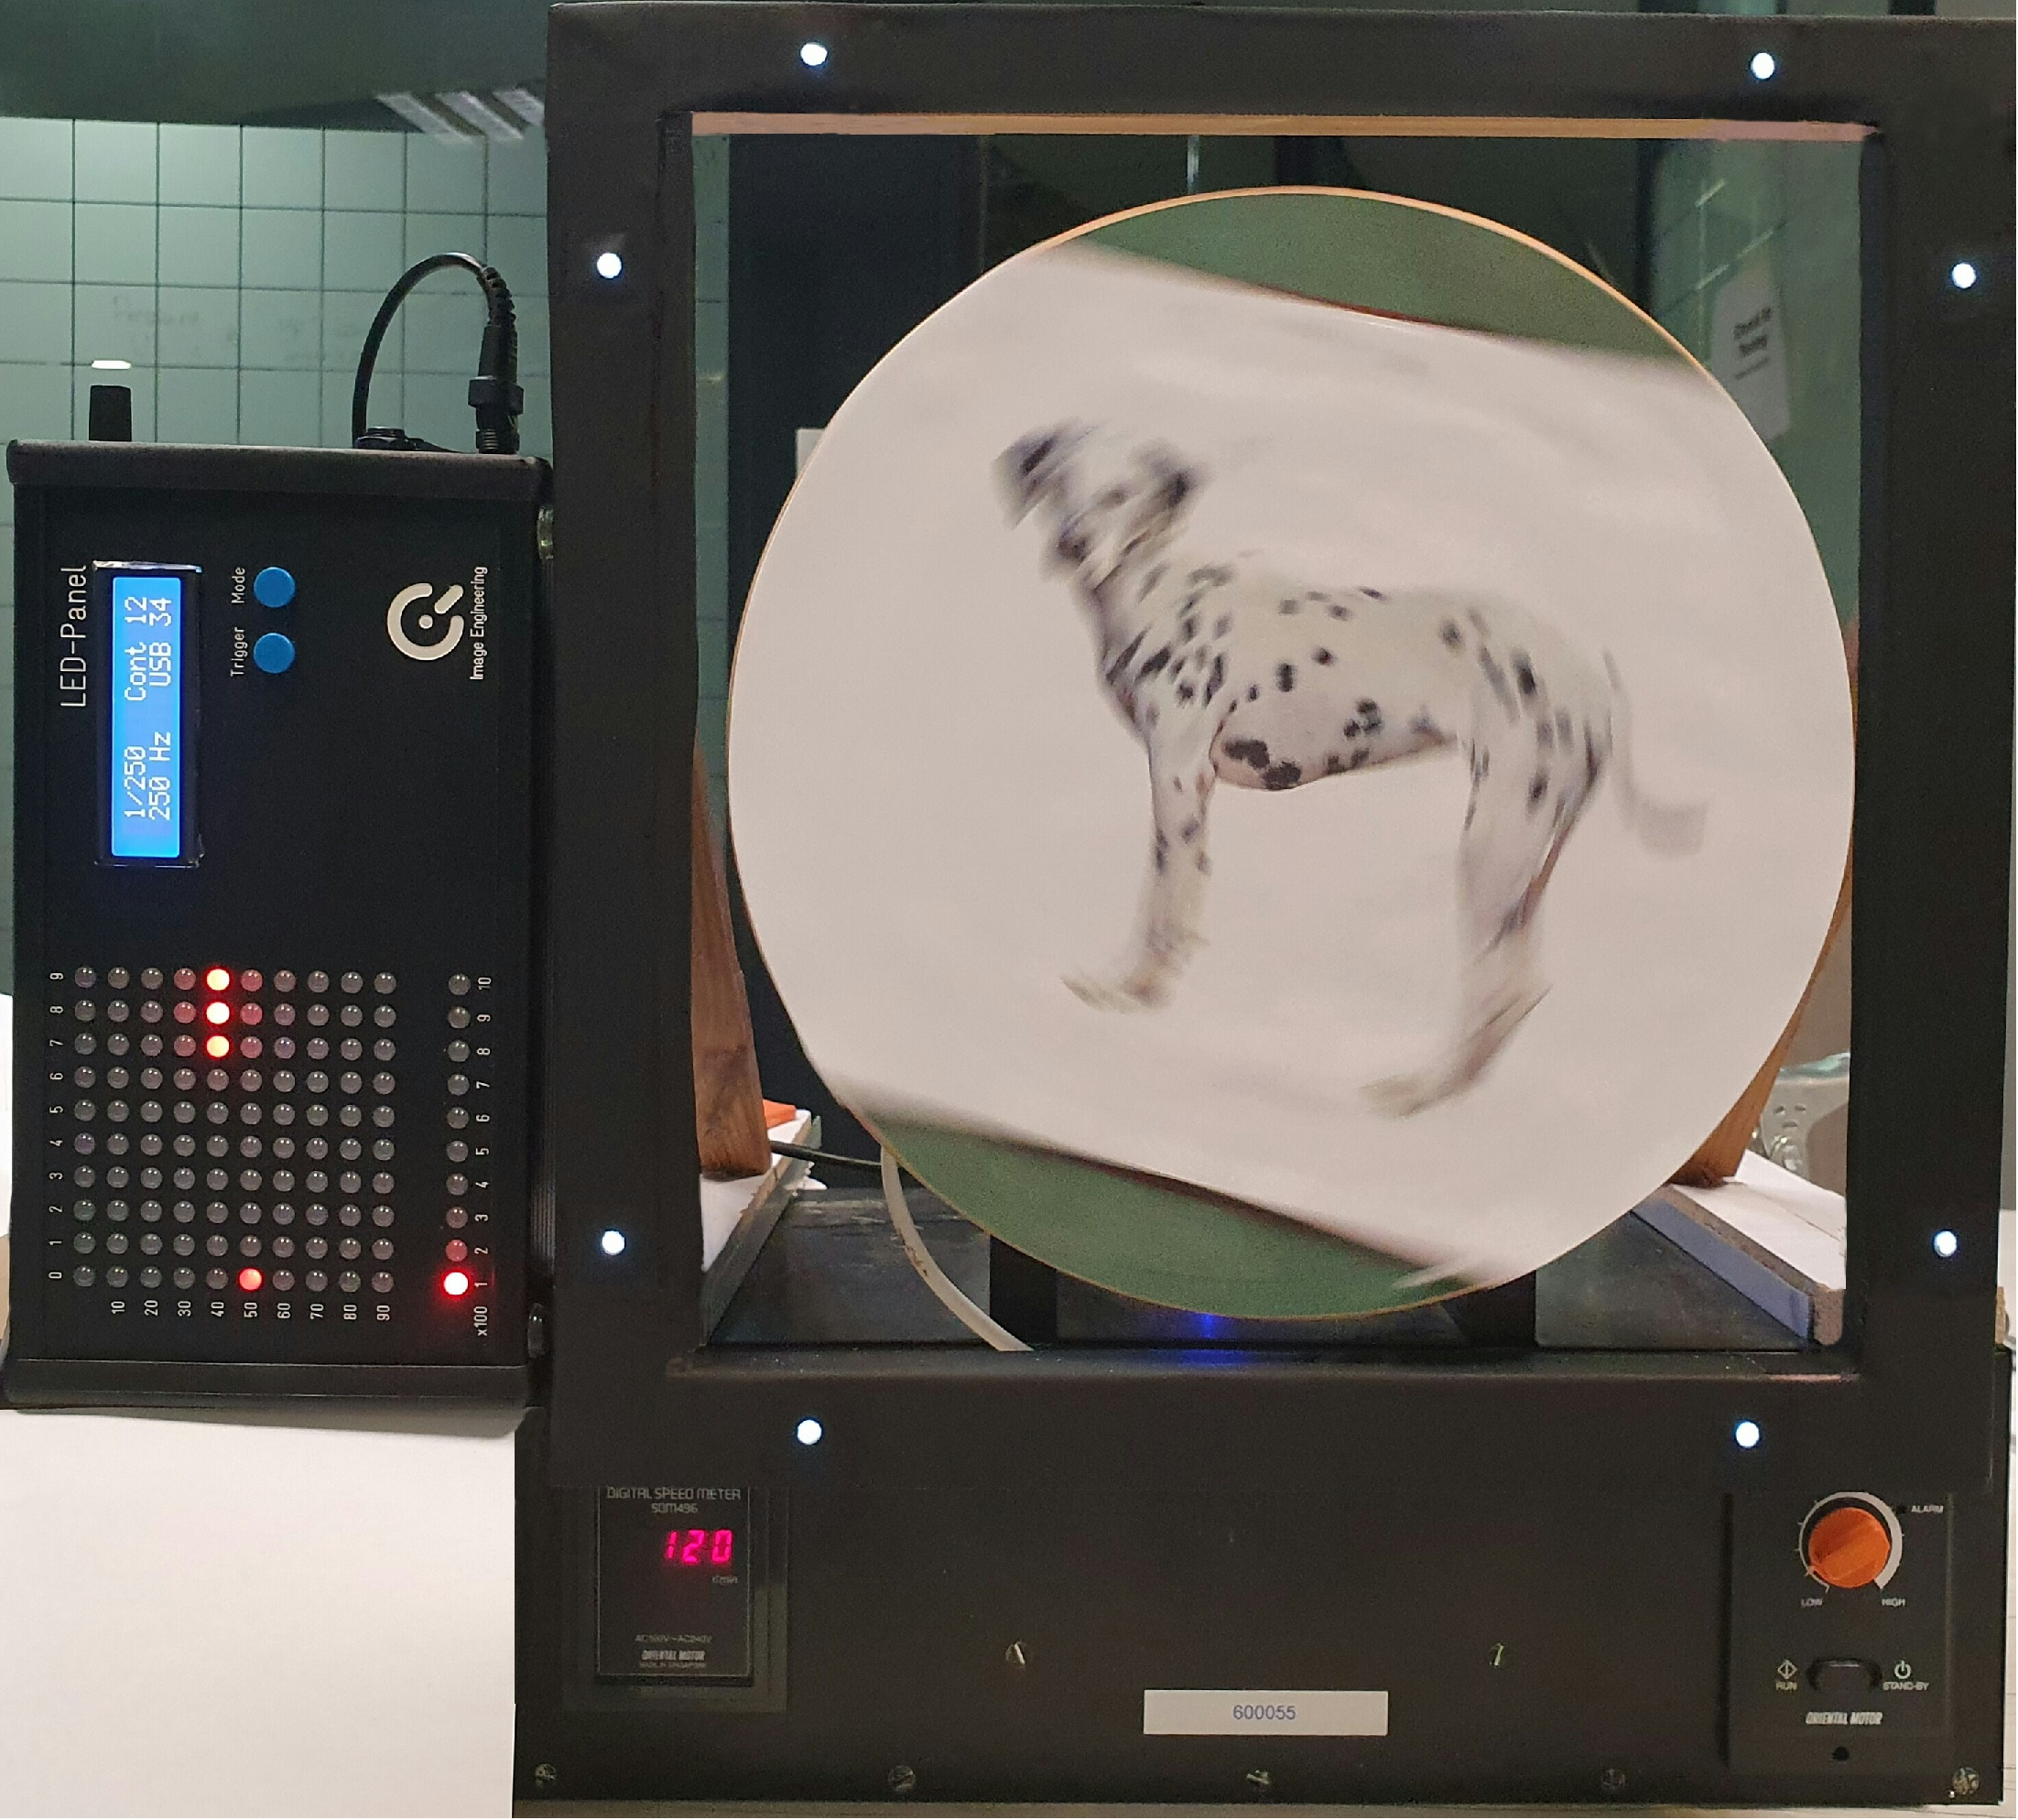
\includegraphics[width=0.25\linewidth]{images/EFI_NET_SETUP.jpg}
				\end{figure}
				\item Dataset introduced in \footfullcite{mueggler2017event}, by a DAVIS240 camera.
				\begin{figure}
					\centering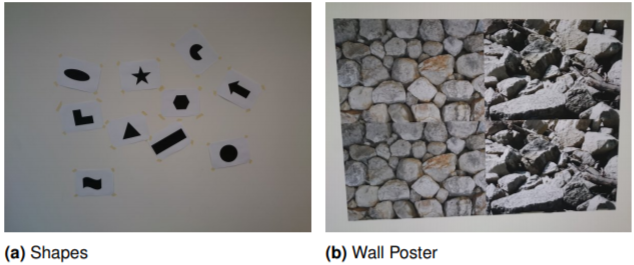
\includegraphics[width=0.5\linewidth]{images/scene_dataset.png}
				\end{figure}
			\end{itemize}
		}
		\only<3>{
			Quatitative results
			\begin{itemize}
				\item Comparison on public dataset\footfullcite{mueggler2017event}\\
				\begin{figure}
					\centering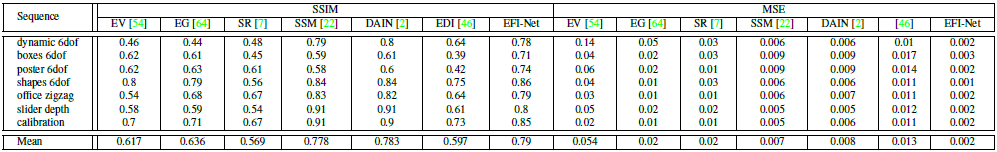
\includegraphics[width=0.98\linewidth]{images/EFI_NET_quatitative_results_one.png}
				\end{figure}
				\item Comparison on self-collected dataset\\
				\begin{figure}
					\centering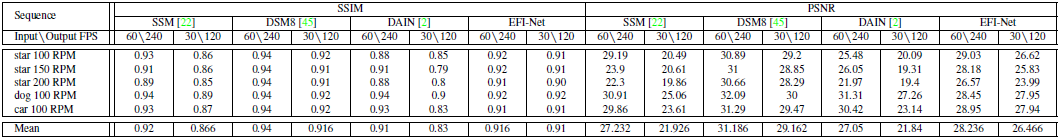
\includegraphics[width=0.98\linewidth]{images/EFI_NET_quatitative_results_two.png}
				\end{figure}
			\end{itemize}
		}
		\only<4>{
			Qualitative results
			\begin{figure}
				\centering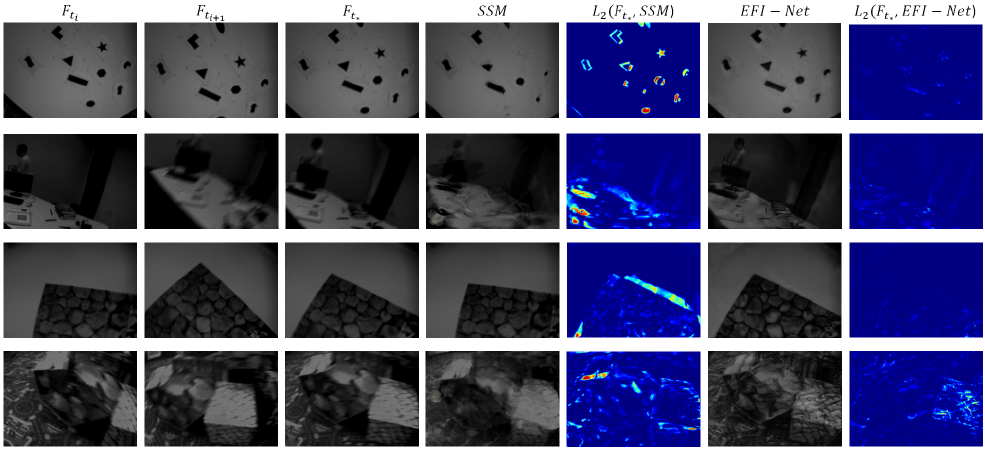
\includegraphics[width=0.95\linewidth]{images/EFI_NET_qualitative_results_one.png}
			\end{figure}
			\centering {\small Comparison with SSM\footfullcite{jiang2018super} on the dataset\footfullcite{mueggler2017event}}
		}
		\only<5>{
			Qualitative results
			\begin{figure}
				\centering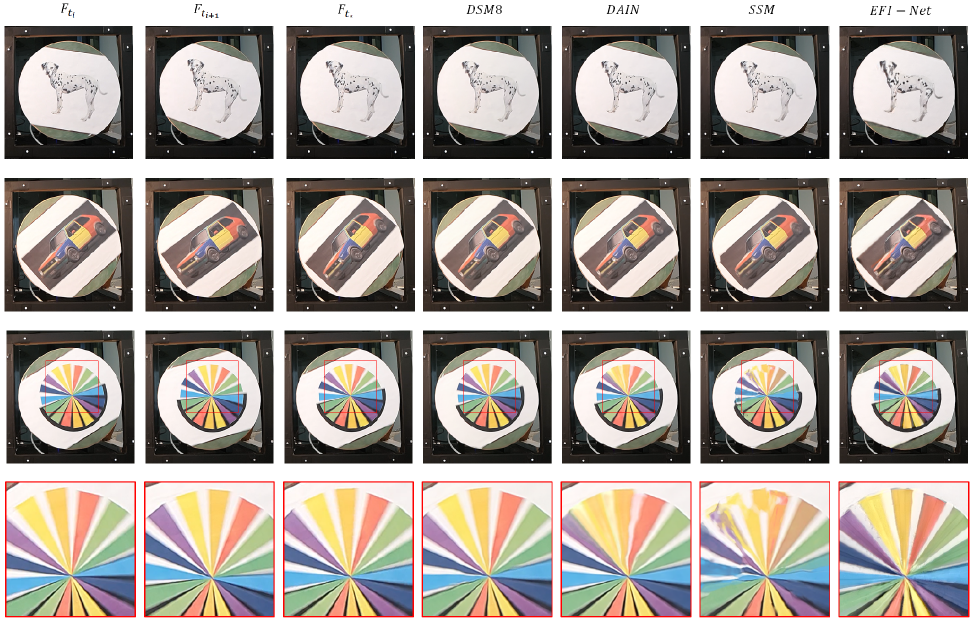
\includegraphics[width=0.95\linewidth]{images/EFI_NET_qualitative_results_two.png}
			\end{figure}		
		}
	\end{frame}

	\begin{frame}{Conclusions}
		\begin{figure}
			\centering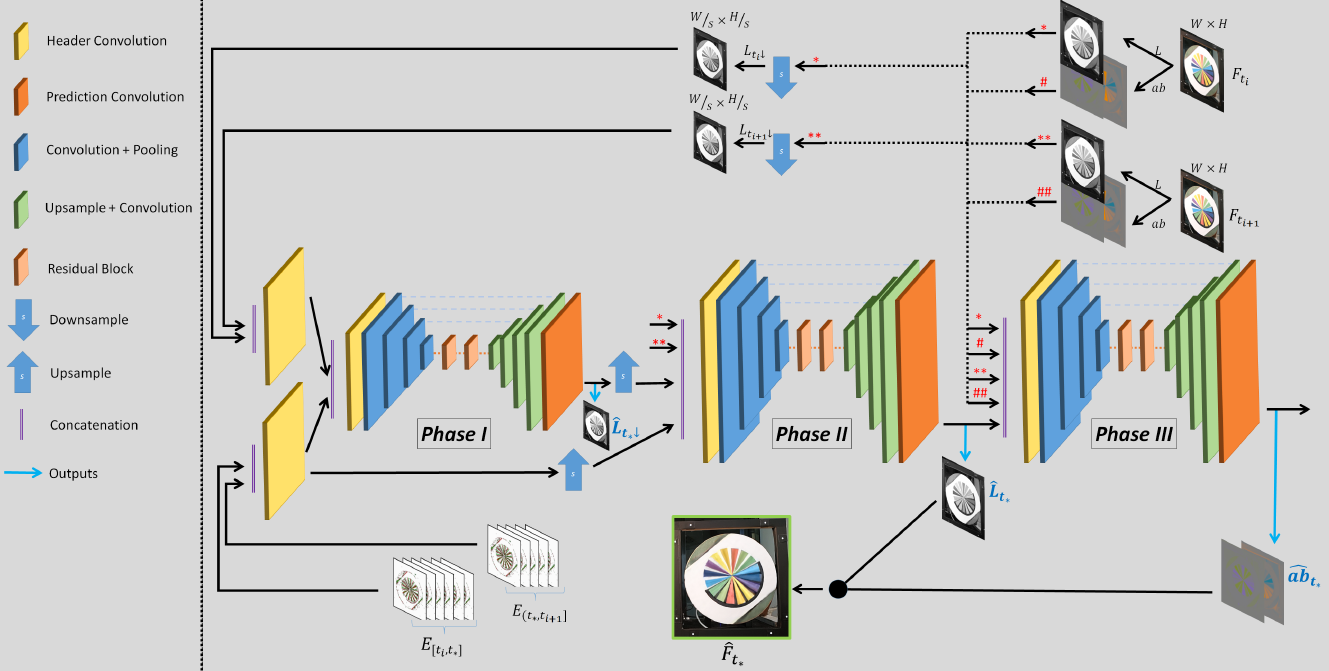
\includegraphics[width=0.85\linewidth]{images/EFI_NET_architecture.png}
		\end{figure}
		\begin{itemize}
			\item Propose a \alert{fusion pipeline}, combine conventional frames with \alert{events} for \textit{VFI}.
			\item \alert{Simulate events} in a simple way, and verify the \alert{generalization} to multiple dataset.
			\item \alert{Contribute a novel dataset} with spatio-temporal alignment of frames and events.
		\end{itemize}
	\end{frame}

	\section{Paper 2: Time Lens: Event-based Video Frame Interpolation}
	\begin{frame}{Paper 2: Time Lens\textit{(CVPR2021)}}
		\begin{figure}
			\centering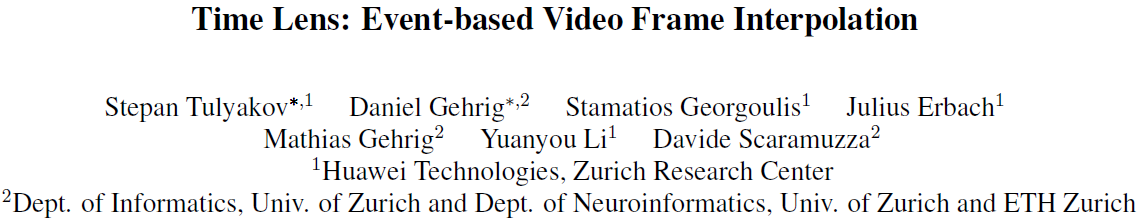
\includegraphics[width=0.95\linewidth]{images/Time_Lens_paper.png}
		\end{figure}
	\end{frame}
	
	\begin{frame}{Motivation}
		\begin{itemize}
			\item Warping-based methods: compute \alert{optical flow} to \alert{warp input frames}, can't solve \alert{non-linear motion}.
			\item Event-based methods: learn \alert{frame residual}, can't solve \alert{low-texture surface}.
			\begin{figure}
				\centering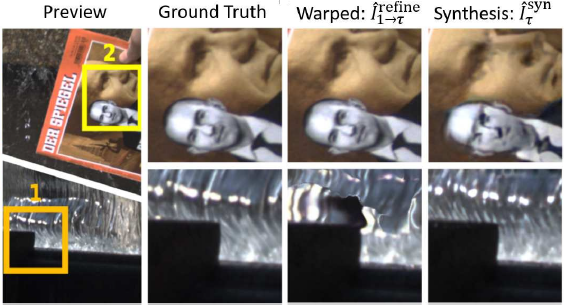
\includegraphics[width=0.7\linewidth]{images/warping_based_vs_event_based.png}
			\end{figure}
			\item<2> Warping-based and Event-based methods each has its advantages and disadvantages, so we can \alert{complement} both methods.
		\end{itemize}
	\end{frame}

	\begin{frame}{Problem Formulation}
		Input: left $ I_0 $  and right $ I_1 $ RGB frames, and the left $ E_{0 \rightarrow \tau} $ and right $ E_{1 \rightarrow \tau} $ event sequences.
		\begin{figure}
			\centering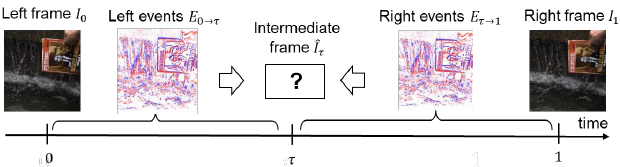
\includegraphics[width=0.8\linewidth]{images/problem formulation.png}
		\end{figure}
		Output: interpolate $ \hat{I}_{\tau} $ at random timestamp
	\end{frame}

	\begin{frame}{Proposed Method}
		\only<1>{
			WorkFlow
			\begin{figure}
				\centering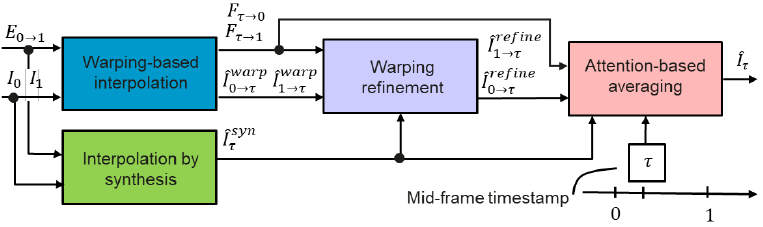
\includegraphics[width=0.8\linewidth]{images/Time_lens_workflow.png}
			\end{figure}
			\begin{enumerate}
				\item Warping-based interpolation: use \alert{events} to compute flow, and \alert{warp input frames}
				\item Interpolation by synthesis: \alert{fuse} frames and events
				\item Warping refinement module: compute \alert{residual flow} to refine
				\item Attention-based averaging: combine warping-based and synthesis-based results
			\end{enumerate}		
		}
		\only<2-3>{
			Warping-based interpolation
			\begin{figure}
				\centering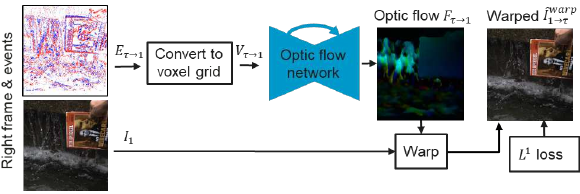
\includegraphics[width=0.6\linewidth]{images/Warping-based interpolation.png}
			\end{figure}
			\begin{itemize}
				\item Event representation: convert to voxel grid
				\only<2>{
					\begin{figure}
						\centering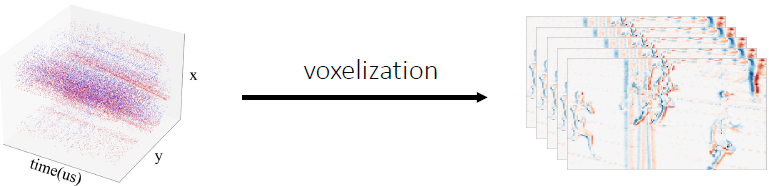
\includegraphics[width=0.6\linewidth]{images/voxelization.png}
					\end{figure}
				}
				\only<3>{
					\item Estimate optical flow by events $ E_{\tau \rightarrow 0} $ and $ E_{\tau \rightarrow 1} $
					\item Warp the input frames
					\item Loss Function: $ \mathcal{L}_{1} $ loss
				}
			\end{itemize}
		}
		\only<4-5>{
			\only<4>{
				WorkFlow
				\begin{figure}
					\centering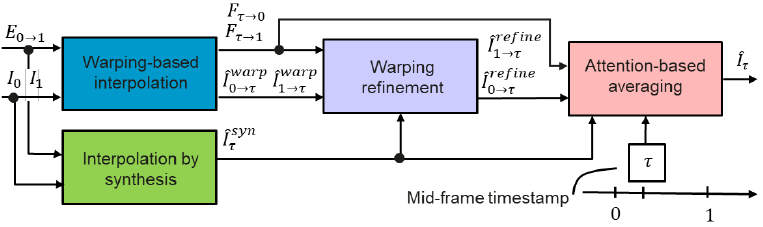
\includegraphics[width=0.8\linewidth]{images/Time_lens_workflow.png}
				\end{figure}
			}
			\only<5>{
				Interpolation by synthesis
				\begin{figure}
					\centering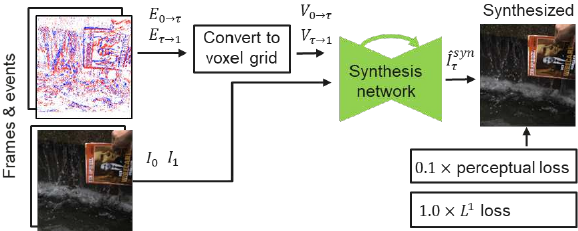
\includegraphics[width=0.6\linewidth]{images/Interpolation by synthesis.png}
				\end{figure}
				\begin{itemize}
					\item Event representation: convert to voxel grid
					\item Synthesis $ I_0,\ I_1,\ V_{0 \rightarrow \tau},\ V_{\tau \rightarrow 1} $ directly
					\item Loss Functions: $ 0.1 \times $perceptual loss $ +\ 1.0 \times \mathcal{L}_{1} $ loss 
				\end{itemize}
			}
			
		}
		\only<6-7>{
			\only<6>{
				WorkFlow
				\begin{figure}
					\centering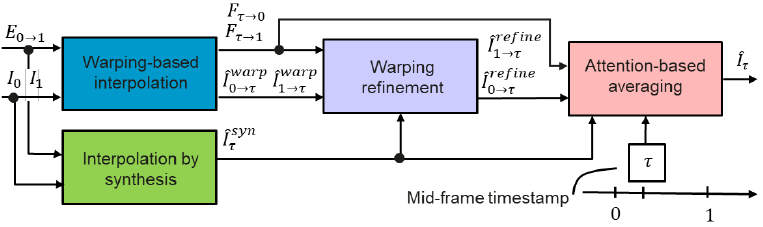
\includegraphics[width=0.8\linewidth]{images/Time_lens_workflow.png}
				\end{figure}
			}		
			\only<7>{
				Warping refinement
				\begin{figure}
					\centering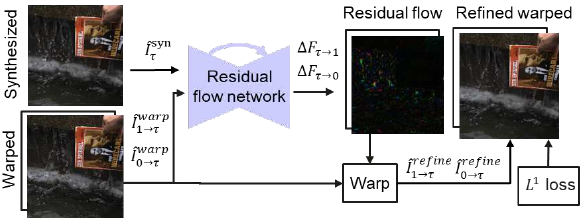
\includegraphics[width=0.6\linewidth]{images/Warping refinement.png}
				\end{figure}
				\begin{itemize}
					\item Compute residual flow $ \Delta F_{\tau \rightarrow 0}$ and $ \Delta F_{\tau \rightarrow 1} $
					\item Warp $ \hat{I}_{0 \rightarrow \tau}^{warp} $ and $ \hat{I}_{1 \rightarrow \tau}^{warp} $ by residual flow
					\item Loss Function: $ \mathcal{L}_{1} $ loss
				\end{itemize}
			}
		}
		\only<8-9>{
			\only<8>{
				WorkFlow
				\begin{figure}
					\centering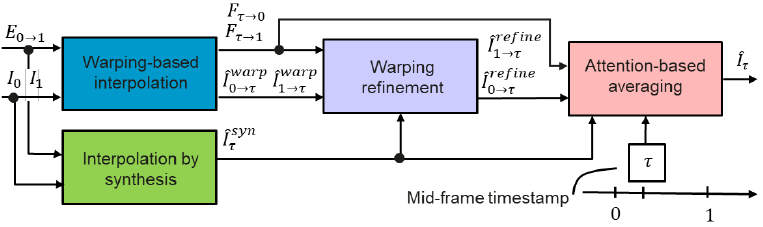
\includegraphics[width=0.8\linewidth]{images/Time_lens_workflow.png}
				\end{figure}
			}	
			\only<9>{
				Attention Averaging
				\begin{figure}
					\centering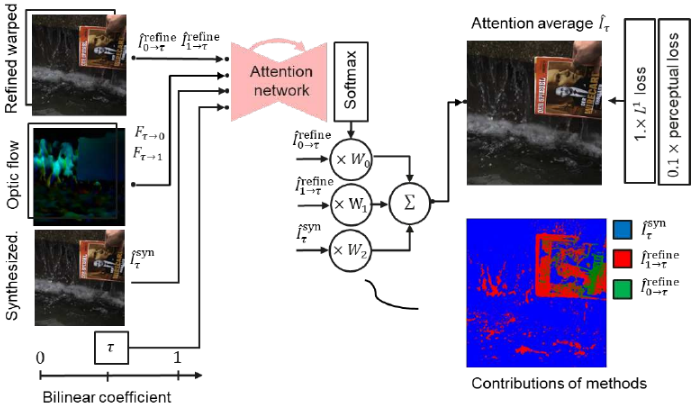
\includegraphics[width=0.65\linewidth]{images/attention averaging.png}
				\end{figure}
				\begin{itemize}
					\item Compute blending coefficients, via $ \hat{I}_{0 \rightarrow \tau}^{\text {refine }},\ \hat{I}_{1 \rightarrow \tau}^{\text {refine }}$ and $ \hat{I}^{\text {syn }} $, $ F_{\tau \rightarrow 0} $, $ F_{\tau \rightarrow 1} $ and bi-linear coefficient $ \tau $, which depends on the new frame position.
					\item Blend $ \hat{I}_{0 \rightarrow \tau}^{\text {refine }},\ \hat{I}_{1 \rightarrow \tau}^{\text {refine }}$ and $ \hat{I}^{\text {syn }} $
				\end{itemize}
			}
		}
	\end{frame}

	\begin{frame}{Experiments}
		Training Details:
		\begin{itemize}
			\item Training Dataset: \textit{Vimeo90k} septuplet dataset\footfullcite{xue2019video} frames, and its \alert{systhetic events}.
			\only<1>{
				\begin{figure}
					\centering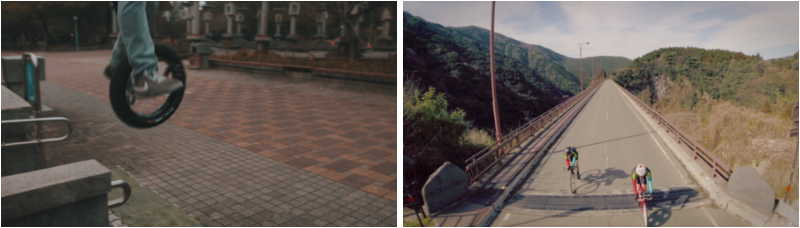
\includegraphics[width=0.7\linewidth]{images/vimeo90k.png}
				\end{figure}
			}
			\only<2>{
				\begin{figure}
					\centering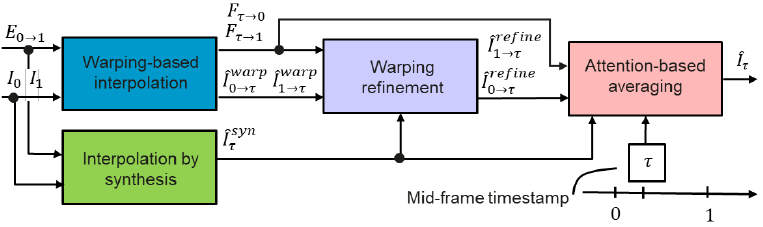
\includegraphics[width=0.7\linewidth]{images/Time_lens_workflow.png}
				\end{figure}
			}
			\only<2>{
				\item Training Process: synthesis-based interpolation $ \rightarrow $ warping-based interpolation $ \rightarrow $ warping refinement $ \rightarrow $ attention averaging module.
			}
		\end{itemize}
	\end{frame}

	\begin{frame}{Experiments}
		Testing Benchmarking:
		\begin{itemize}
			\item Synthetic datasets: \textit{Vimeo90k}\footfullcite{xue2019video} and \textit{Middlebury}\footfullcite{baker2011database}, skip 1 or 3 frames and reconstruct them.
			\item High Quality Frames(HQF)\footfullcite{stoffregen2020reducing} dataset: \alert{video$ \& $events} dataset, without blur and saturation, collected by DAVIS240.
			\item<2> High Speed Event-RGB dataset: \alert{Self-collected}, \alert{Higher frame rate 225FPS}, \alert{Higher event resolution $ 1280 \times 720 $}.
		\end{itemize}
		\only<2>{
			\begin{figure}
				\centering 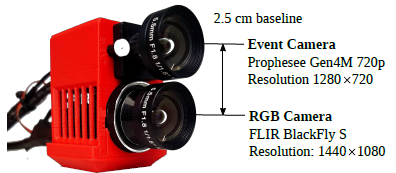
\includegraphics[width=0.5\linewidth]{images/camera.png}
			\end{figure}
		}
	\end{frame}
	
	\begin{frame}{Experiments}
		\only<1>{
			Quatitative results
			\begin{itemize}
				\item Comparison on \textit{Vimeo90k}\footfullcite{xue2019video} and \textit{Middlebury}\footfullcite{baker2011database} dataset\\
				\begin{figure}
					\centering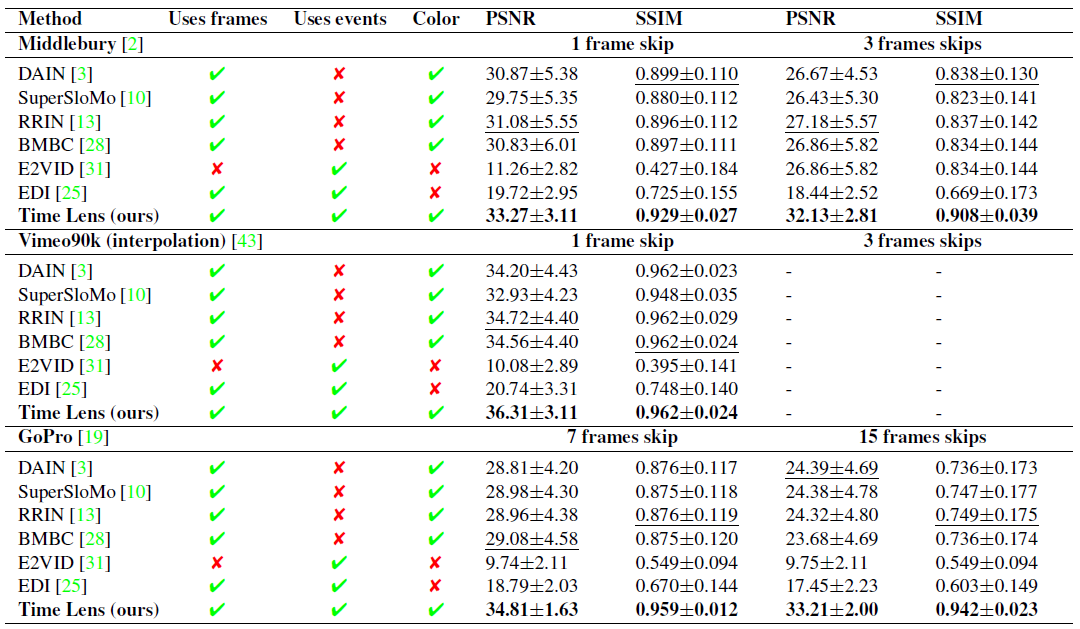
\includegraphics[width=0.95\linewidth]{images/Time_lens_quatitative_results_one.png}
				\end{figure}
			\end{itemize}
		}
		\only<2>{
			Quatitative results
			\begin{itemize}
				\item Comparison on HQF\footfullcite{stoffregen2020reducing} dataset\\
				\begin{figure}
					\centering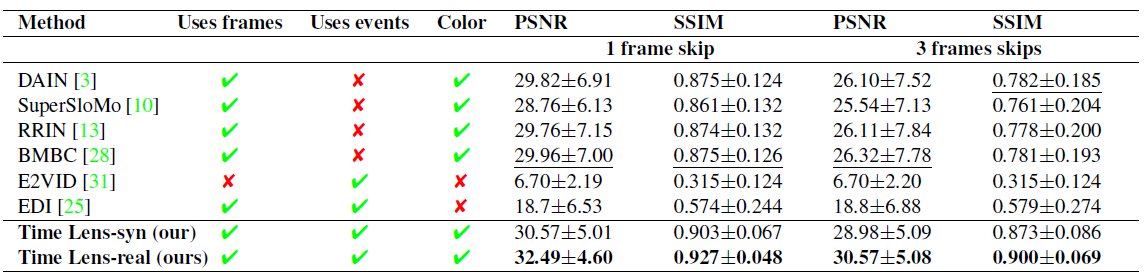
\includegraphics[width=0.95\linewidth]{images/Time_lens_quatitative_results_two.png}
				\end{figure}
				\item \textit{Time Lens-syn}: train only on synthetic data
				\item \textit{Time Lens-real}: train on synthetic data and \alert{fine-tuned} on real event data
			\end{itemize}
		}
		\only<3>{
			Quatitative results
			\begin{itemize}
				\item Comparison on HS-ERGB(self-collected) dataset\\
				\begin{figure}
					\centering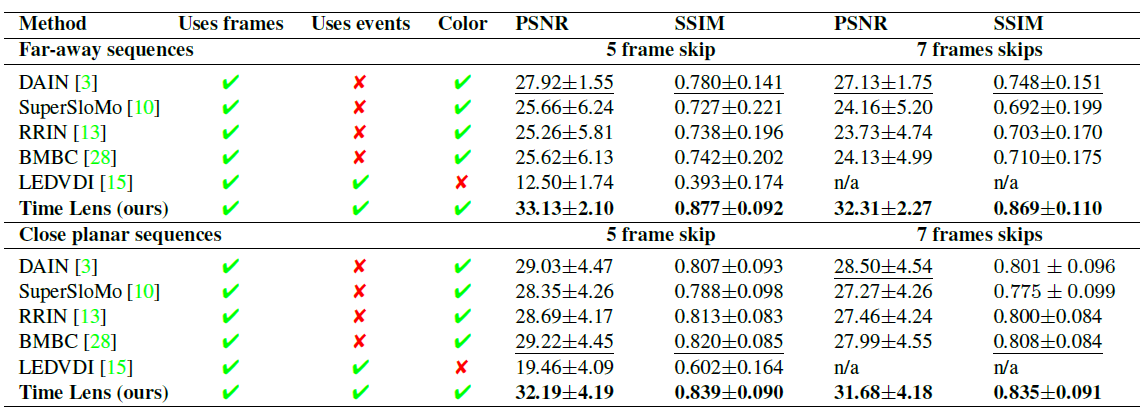
\includegraphics[width=0.95\linewidth]{images/Time_lens_quatitative_results_three.png}
				\end{figure} 
			\end{itemize}
		}
		
		\only<4>{
			Qualitative results
			\begin{figure}
				\centering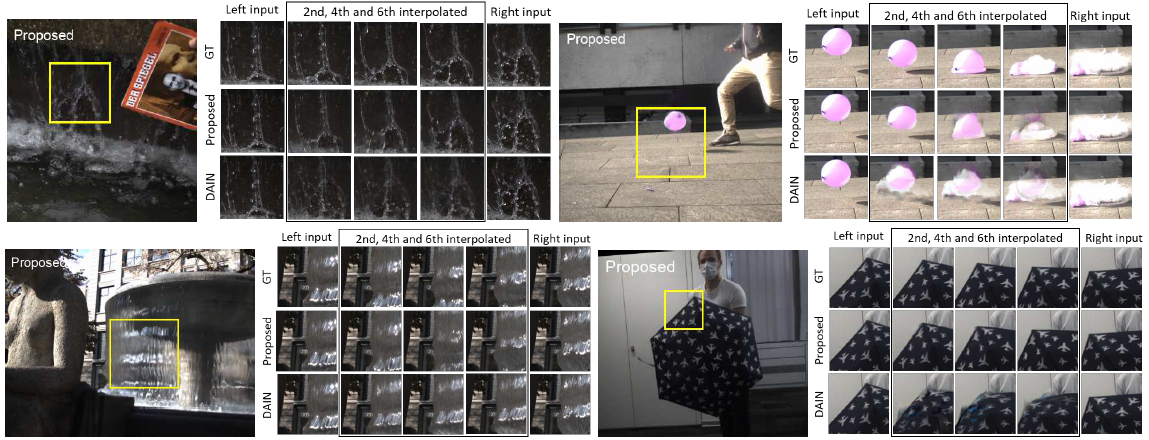
\includegraphics[width=0.95\linewidth]{images/Time_Lens_qualitative_results_one.png}
			\end{figure}
			\centering {\small Comparison on non-linear and complex scenarios}
		}

	\end{frame}

	\begin{frame}{Conclusions}
		\begin{figure}
			\centering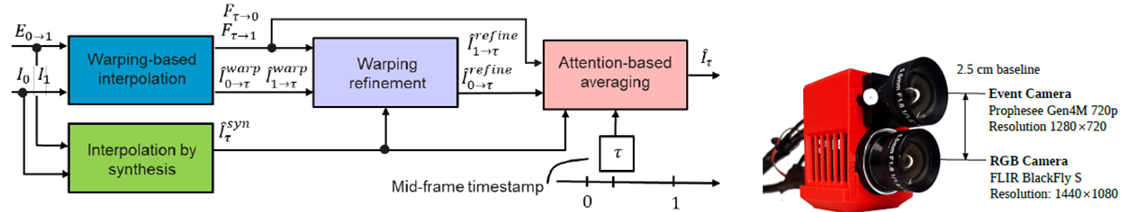
\includegraphics[width=0.85\linewidth]{images/Time_Lens_conclusion.png}
		\end{figure}
		\begin{itemize}
			\item Leverage the advantages of \alert{event-based and flow-based} respectively.
			\item Release a large-scale \alert{HS-ERGB dataset}, pushing the limits of \textit{VFI} in complex scenarios.
		\end{itemize}
	\end{frame}
	
	\begin{frame}{}
		\centering \Huge
		\emph{Thanks,  Q \& A }
	\end{frame}
    
\end{document}